\documentclass[tikz,border=2mm]{standalone}
\usepackage[T1]{fontenc}
\usepackage[swedish,english]{babel}
\usepackage{tikz}
\usetikzlibrary{arrows,positioning}
\usepackage{pgfplots}
\usepackage{amsmath,mathtools}
\usepgfplotslibrary{fillbetween}
\begin{document}
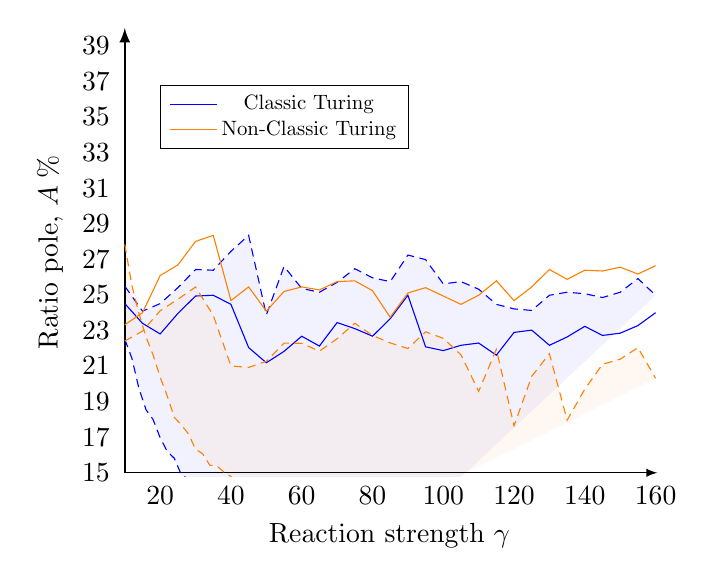
\begin{tikzpicture}
\begin{axis}[
    %hide axis,
    %axis lines* = left,
    %axis lines=left, xtick=\empty, ytick=\empty.
    axis line style={draw=none},
    tick style={draw=none},
    xticklabel style={yshift=-0.1mm},
    xmin = 8.5,
   xmax = 161,
    ymin = 14.8,
    ymax = 40,
    %grid=both,
    %xtick = {1,0.95,...,0.6},
    ytick = {15,17,...,100},    
    %xticklabels = {{zero},$\alpha$,$\varphi$},
   %xlabel style={at={(axis cs:0.61,7)},anchor=east,align=center},
    %ylabel style={at={(axis cs:1.00,35)},anchor=north,rotate=0},
	xlabel = {Reaction strength $\gamma$},
        ylabel = {Ratio pole, $A\;\%$},
    legend style={at={(axis cs:20,35)},anchor=west,cells={align=center},nodes={scale=0.75}},
    %x dir=reverse
    %legend entries = {Decreasing the inactivation rate $k_{-2}$}
]
%-------------------------------------------------------------------------------------------------
% AXES
\draw[->,-latex, thick] (axis cs: 10,15) -- (axis cs: 10,40); % y-axis
\draw[->,-latex] (axis cs: 10,15) -- (axis cs: 160.5,15); % x-axis
%-------------------------------------------------------------------------------------------------
%-------------------------------------------------------------------------------------------------
% Classical 
%-------------------------------------------------------------------------------------------------
\addplot[forget plot,densely dashed,color=blue,name path=UpratioPoleClassical] coordinates {
		(10.0000	,	25.4902	)
		(15.0000	,	24.0835	)
		(20.0000	,	24.5098	)
		(25.0000	,	25.4049	)
		(30.0000	,	26.4280	)
		(35.0000	,	26.3853	)
		(40.0000	,	27.4510	)
		(45.0000	,	28.3461	)
		(50.0000	,	23.8704	)
		(55.0000	,	26.5985	)
		(60.0000	,	25.3623	)
		(65.0000	,	25.1492	)
		(70.0000	,	25.7033	)
		(75.0000	,	26.4706	)
		(80.0000	,	25.9591	)
		(85.0000	,	25.7460	)
		(90.0000	,	27.2379	)
		(95.0000	,	26.9821	)
		(100.0000	,	25.6181	)
		(105.0000	,	25.7460	)
		(110.0000	,	25.3197	)
		(115.0000	,	24.4672	)
		(120.0000	,	24.2114	)
		(125.0000	,	24.1262	)
		(130.0000	,	24.9787	)
		(135.0000	,	25.1492	)
		(140.0000	,	25.0639	)
		(145.0000	,	24.8508	)
		(150.0000	,	25.1492	)
		(155.0000	,	25.9165	)
		(160.0000	,	24.9787	)
};

\addplot[color=blue] coordinates {
		(10.0000	,	24.5098	)
		(15.0000	,	23.4015	)
		(20.0000	,	22.8048	)
		(25.0000	,	23.9557	)
		(30.0000	,	24.9361	)
		(35.0000	,	24.9787	)
		(40.0000	,	24.4672	)
		(45.0000	,	22.0375	)
		(50.0000	,	21.1850	)
		(55.0000	,	21.8244	)
		(60.0000	,	22.6769	)
		(65.0000	,	22.1228	)
		(70.0000	,	23.4442	)
		(75.0000	,	23.1032	)
		(80.0000	,	22.6769	)
		(85.0000	,	23.6573	)
		(90.0000	,	24.9787	)
		(95.0000	,	22.0801	)
		(100.0000	,	21.8670	)
		(105.0000	,	22.1654	)
		(110.0000	,	22.2933	)
		(115.0000	,	21.6113	)
		(120.0000	,	22.8900	)
		(125.0000	,	23.0179	)
		(130.0000	,	22.1654	)
		(135.0000	,	22.6343	)
		(140.0000	,	23.2310	)
		(145.0000	,	22.7195	)
		(150.0000	,	22.8474	)
		(155.0000	,	23.2737	)
		(160.0000	,	23.9983	)
};

\addplot[forget plot,densely dashed,color=blue,name path=DownratioPoleClassical] coordinates {
		(10.0000	,	22.5064	)
		(12.0000	,	21.4408	)
		(14.0000	,	19.7357	)
		(16.0000	,	18.5422	)
		(18.0000	,	17.9881	)
		(20.0000	,	16.9650	)
		(22.0000	,	16.1978	)
		(24.0000	,	15.8142	)
		(26.0000	,	14.8764	)
		(28.0000	,	14.6633	)
		(30.0000	,	13.8107	)
		(32.0000	,	13.0009	)
		(34.0000	,	12.9582	)
		(36.0000	,	12.4467	)
		(38.0000	,	12.1910	)
		(40.0000	,	11.8073	)
		(42.0000	,	11.0827	)
		(44.0000	,	10.6991	)
		(46.0000	,	10.6991	)
		(48.0000	,	10.6564	)
		(50.0000	,	10.0171	)
		(52.0000	,	9.7613	)
		(54.0000	,	9.5908	)
		(56.0000	,	9.8892	)
		(58.0000	,	9.5482	)
		(60.0000	,	9.2924	)
		(62.0000	,	8.8662	)
		(64.0000	,	8.8235	)
		(66.0000	,	8.4825	)
		(68.0000	,	8.5678	)
		(70.0000	,	8.2268	)
};
\addplot[blue!50,opacity=0.1,forget plot] fill between[of=UpratioPoleClassical and DownratioPoleClassical];

\addlegendentry{Classic Turing}% Add to legend
%-------------------------------------------------------------------------------------------------
% Non-classical
%-------------------------------------------------------------------------------------------------
\addplot[forget plot,densely dashed,color=orange,name path=UpratioPoleNonClassical] coordinates {
		(10.0000	,	27.8346	)
		(12.0000	,	25.5328	)
		(14.0000	,	23.9557	)
		(16.0000	,	22.6343	)
		(18.0000	,	21.6113	)
		(20.0000	,	20.3751	)
		(22.0000	,	19.3095	)
		(24.0000	,	18.1159	)
		(26.0000	,	17.6897	)
		(28.0000	,	17.1782	)
		(30.0000	,	16.3257	)
		(32.0000	,	16.0699	)
		(34.0000	,	15.4305	)
		(36.0000	,	15.3879	)
		(38.0000	,	15.0469	)
		(40.0000	,	14.7911	)
		(42.0000	,	14.2370	)
		(44.0000	,	14.2370	)
		(46.0000	,	13.9812	)
		(48.0000	,	13.5976	)
		(50.0000	,	13.2992	)
		(52.0000	,	12.7877	)
		(54.0000	,	12.8730	)
		(56.0000	,	12.7451	)
		(58.0000	,	12.7025	)
		(60.0000	,	12.1483	)
		(62.0000	,	12.1483	)
		(64.0000	,	11.8073	)
		(66.0000	,	12.1057	)
		(68.0000	,	11.5942	)
		(70.0000	,	11.3811	)
};

\addplot[color=orange] coordinates {
		(10.0000	,	23.3163	)
		(15.0000	,	23.9983	)
		(20.0000	,	26.0870	)
		(25.0000	,	26.6837	)
		(30.0000	,	28.0051	)
		(35.0000	,	28.3461	)
		(40.0000	,	24.6803	)
		(45.0000	,	25.4476	)
		(50.0000	,	24.0835	)
		(55.0000	,	25.1918	)
		(60.0000	,	25.4476	)
		(65.0000	,	25.2771	)
		(70.0000	,	25.7460	)
		(75.0000	,	25.7886	)
		(80.0000	,	25.2344	)
		(85.0000	,	23.7425	)
		(90.0000	,	25.1066	)
		(95.0000	,	25.4049	)
		(100.0000	,	24.9361	)
		(105.0000	,	24.4672	)
		(110.0000	,	24.9787	)
		(115.0000	,	25.7886	)
		(120.0000	,	24.6803	)
		(125.0000	,	25.4476	)
		(130.0000	,	26.4280	)
		(135.0000	,	25.8738	)
		(140.0000	,	26.3853	)
		(145.0000	,	26.3427	)
		(150.0000	,	26.5558	)
		(155.0000	,	26.1722	)
		(160.0000	,	26.6411	)
};

\addplot[forget plot,densely dashed,color=orange,name path=DownratioPoleNonClassical] coordinates {
		(10.0000	,	22.4041	)
		(15.0000	,	22.9625	)
		(20.0000	,	24.1091	)
		(25.0000	,	24.7528	)
		(30.0000	,	25.4433	)
		(35.0000	,	23.8534	)
		(40.0000	,	21.0060	)
		(45.0000	,	20.9207	)
		(50.0000	,	21.2660	)
		(55.0000	,	22.2890	)
		(60.0000	,	22.2762	)
		(65.0000	,	21.8372	)
		(70.0000	,	22.5362	)
		(75.0000	,	23.4058	)
		(80.0000	,	22.7153	)
		(85.0000	,	22.3018	)
		(90.0000	,	21.9864	)
		(95.0000	,	22.9241	)
		(100.0000	,	22.5575	)
		(105.0000	,	21.6326	)
		(110.0000	,	19.5823	)
		(115.0000	,	21.9395	)
		(120.0000	,	17.6428	)
		(125.0000	,	20.4263	)
		(130.0000	,	21.6922	)
		(135.0000	,	17.9582	)
		(140.0000	,	19.7059	)
		(145.0000	,	21.0997	)
		(150.0000	,	21.3853	)
		(155.0000	,	22.0332	)
		(160.0000	,	20.3154	)
};
\addplot[orange!50,opacity=0.1,forget plot] fill between[of=UpratioPoleNonClassical and DownratioPoleNonClassical];

\addlegendentry{Non-Classic Turing}% Add to legend
\end{axis}

\end{tikzpicture}



\end{document}
